%\documentclass{bs-exercise}
\documentclass[answers]{exercise}
%\documentclass[additions]{exercise}
%\documentclass[additions,answers]{exercise}


%%%%%%%%%%%%%%%%%%%%%%%%%%%%%%%%%%%%%%%%%%%%%%%%%%%%%%%%%%%%%%%%%%%%%%%%
\bsauthor{Granitzer}
\bsyear{2012}
\bsreadingtitle{Medientechnik}
\usepackage{amsmath}
\usepackage{listings}

\usepackage{color}
\definecolor{gray}{rgb}{0.4,0.4,0.4}
\definecolor{darkblue}{rgb}{0.0,0.0,0.6}
\definecolor{cyan}{rgb}{0.0,0.6,0.6}

\lstset{
  basicstyle=\ttfamily,
  columns=fullflexible,
  showstringspaces=false,
  commentstyle=\color{gray}\upshape
}

\lstdefinelanguage{SVG}
{
  morestring=[b]",
  morestring=[s]{>}{<},
  morecomment=[s]{<?}{?>},
  stringstyle=\color{black},
  identifierstyle=\color{darkblue},
  keywordstyle=\color{red},
  morekeywords={transform,stroke,path,width,height,d}% list your attributes here
}
\lstdefinelanguage{XML}
{
  morestring=[b]",
  morestring=[s]{>}{<},
  morecomment=[s]{<?}{?>},
  stringstyle=\color{black},
  identifierstyle=\color{darkblue},
  keywordstyle=\color{red},
  morekeywords={xmlns,version,type}% list your attributes here
}



%%%%%%%%%%%%%%%%%%%%%%%%%%%%%%%%%%%%%%%%%%%%%%%%%%%%%%%%%%%%%%%%%%%%%%%%
\begin{document}


%%% These exercises are included in part-ml-basics
\exerciseheader[\today]{�bungsblatt 6 - Vektorgrafik und SVG}


\vspace{2cm} 
\section*{Informationen zum Bonuspunktesystem:} 
�ber Kleinprojekte sowie durch L�sen und Pr�sentieren von einzelnen �bungsaufgaben in den �bungsstunden k�nnen Sie sich Bonuspunkte f�r die Klausur erarbeiten. Die Klausur umfasst 60 Punkte. Maximal 15 Bonuspunkte k�nnen Sie sich f�r die Klausur anrechnen lassen. Der Arbeitsaufwand sollte in etwa 1 ECTS, d.h. 30 Arbeitsstunden umfassen und einen nachhaltigen Lerneffekt f�r die Klausur erzielen. \\

Die einzelnen �bungsaufgaben werden in der jeweiligen �bungseinheit besprochen und auf Basis freiwilliger Meldungen unter den Studierenden verteilt. Die Pr�sentation der Ausarbeitung erfolgt in der n�chsten �bungsstunde.\\

\section*{Aufgaben} 



\begin{exercise}{Bezier Kurven- 4 Pkt.}
\label{ex-de-mt-bezier-002}
Erkl�ren sie den Algorithmus zum Zeichnen von Bezierkurven. Konstruieren sie f�r folgende drei Mengen an St�tzpunkten jeweils 3 Punkte auf der Bezierkurve. Nehmen sie dabei das SVG Koordinatensystem an.

\begin{itemize}
  \item $P=\{(1,1),(3,3)\}$
  \item $P=\{(1,1),(3,3),(1,4)\}$
  \item $P=\{(1,1),(3,3),(1,4),(2,5)\}$
\end{itemize}

Welche Ordnung haben die Bezierkurven?

\answer{
n-1 ter Ordnung
\begin{itemize}
  \item 1-ter Ordnung (gerade)
  \item 2-ter Ordnung
  \item 3-ter Ordnung 
\end{itemize}

SVG-Koordinatensystem: Links Oben.\\

Demo Applet f�r die Punkte (inkl. Source-Code): \url{http://codepen.io/tholman/pen/foxtn}


}

\end{exercise}





\begin{exercise}{Clipping - 4 Pkt.}
\label{ex-de-mt-clipping-002}
Erkl�ren sie den Prozess des Clippings. \\
Gegeben sei folgende Szene, angegeben als Menge primitiver Objekte im SVG Koordinatensystem:  
\begin{itemize}
  \item $G_1=(1,2,12,15)$
  \item $G_2=(6,6,8,9)$
  \item $G_3=(2,12,15,1)$
  \item $R_1=(1,2,13,11)$
  \item $R_2=(4,6,9,2)$
\end{itemize}
Zeichnen sie die Szene im Weltkoordinatensystem und f�hren sie danach ein 
Clipping f�r das Rechteck $(5,5,5,5)$ unter Verwendung des Linien-Clipping Algorithmus von Cohen und Sutherland durch. 
\\

Bemerkung: Rechtecke sind in der Form $R=(x_0,y_0,Breite,H\"ohe)$ gegeben und Geraden als $G=(x_0,y_0,x_1,y_1)$. 

\answer{
Gezeichnete Szene:\\

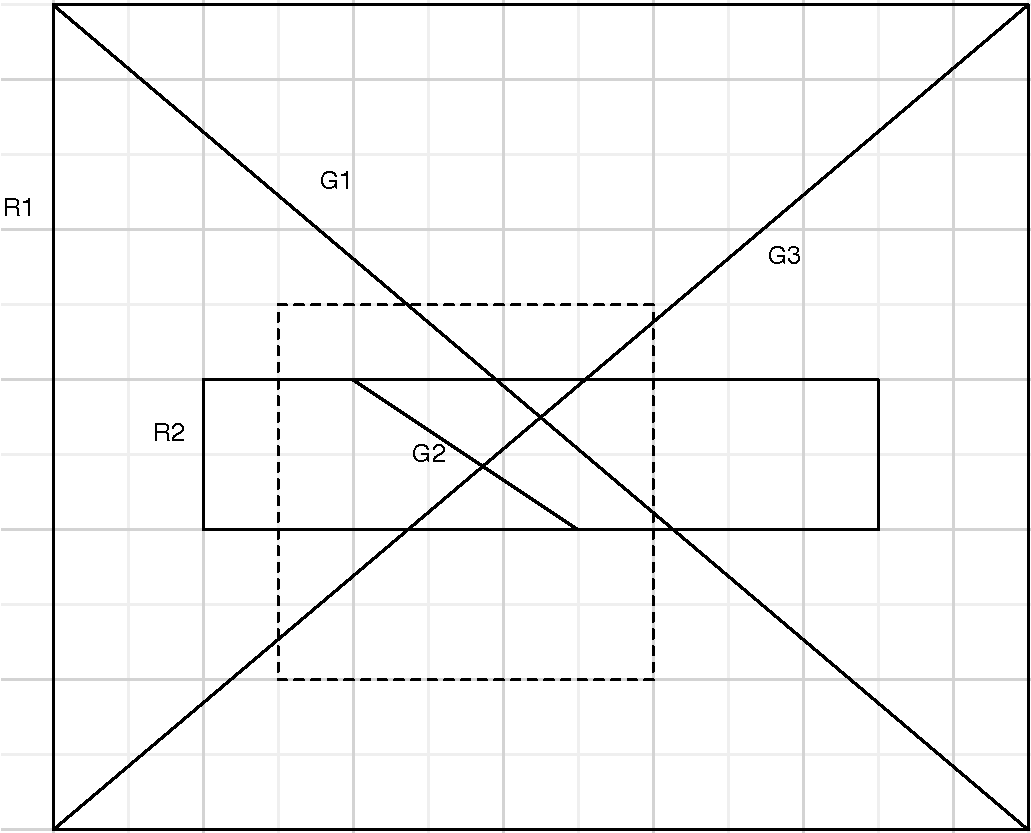
\includegraphics[width=0.5\textwidth]{figure/clipping-ohne}

Clipping Bitbelegung:\\
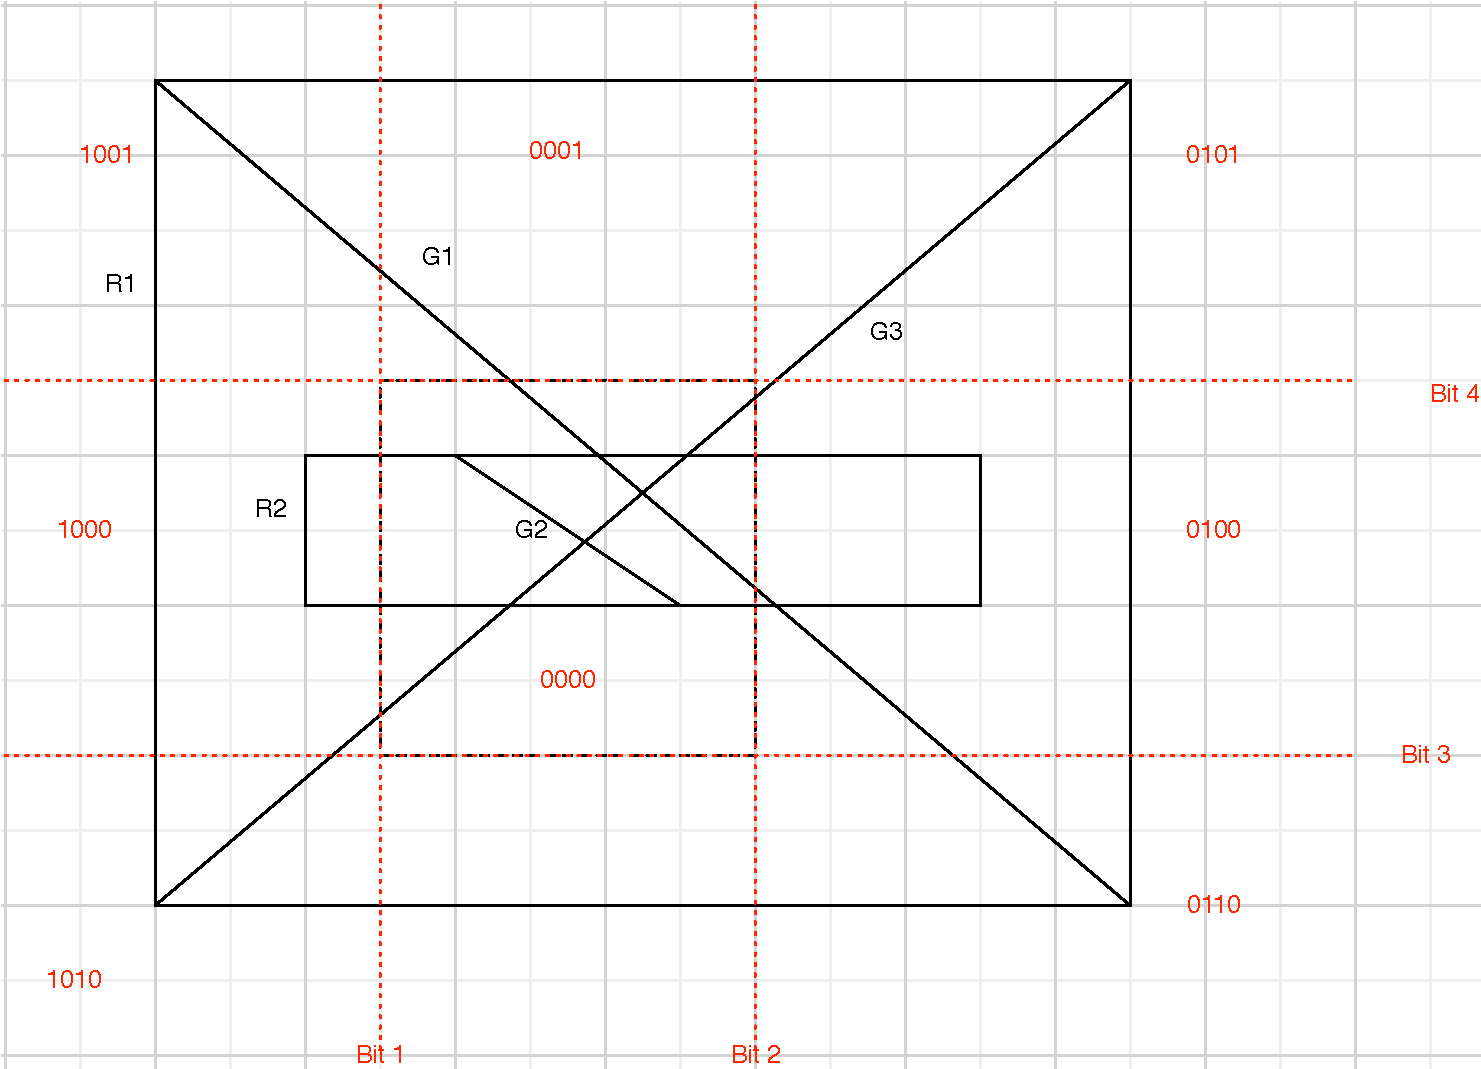
\includegraphics[width=0.5\textwidth]{figure/clipping-mit}

Wenn Linien $P_1\;OR\;P_2=0000$, dann ist diese im Clipping Fenster\\
 
Wenn Linien $P_1\;AND\;P_2\neq 0000$, dann ist diese Linie in den Randbereichen und nicht zu zeichnen.\\

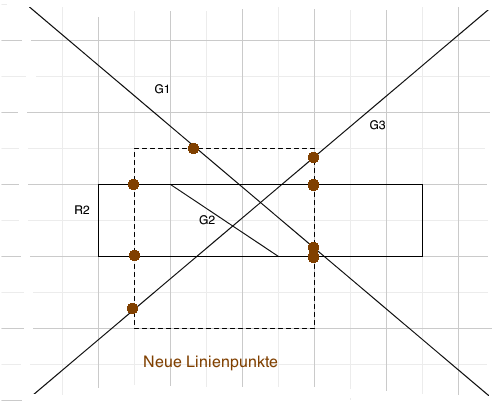
\includegraphics[width=0.5\textwidth]{figure/clipping-final}

}


\end{exercise}


 


\begin{exercise}{SVG Scalable Vector Graphics - 4 Pkt.}
\label{ex-de-mt-SVG}
Erkl\"aren Sie die Elemente und Attribute der folgenden SVG Grafiken und skizzieren sie das Ergebnis.

\begin{enumerate}
  \item Listing 1: Gradient
  {\small
  \lstset{language=SVG}
  \lstinputlisting{figure/gradient.svg}
  } 
  
  \answer{
  \url{http://www.w3schools.com/svg/tryit.asp?filename=trysvg_linear}
  \begin{itemize}
    \item The id attribute of the <linearGradient> tag defines a unique name for the gradient
    \item     The x1, x2, y1,y2 attributes of the <linearGradient> tag define the start and end position of the gradient
    \item The color range for a gradient can be composed of two or more colors. Each color is specified with a <stop> tag. The offset attribute is used to define where the gradient color begin and end
    \item The fill attribute links the ellipse element to the gradient
  \end{itemize}
  }
  \item Listing 2: Animation
  {\small
  \lstset{language=SVG}
  \lstinputlisting{figure/color-animation.svg}
  } 
  \answer{
  \url{http://www.w3schools.com/svg/tryit.asp?filename=animatecolor_1&type=svg}
  \begin{itemize}
    \item three rectangles that change color
    \item animateColor specified by id, change of which attribute over time (attributname,), color and time
    \item time can be set based on properties of other elements
  \end{itemize}
  }
  \item Listing 3: Filter and Definitions
  {\small
  \lstset{language=SVG}
  \lstinputlisting{figure/filter-blur.svg}
  } 
  \item \answer{
  \url{ http://www.w3schools.com/svg/tryit.asp?filename=filter_1&type=svg}
  \begin{itemize}
    \item filterUnits definiert die Art der Gr��enangabe des Filters (Prozent, Pixel etc.)
    \item feGaussianBlur Gau�-Weichzeichner
    \item in selektiert den Kanal (hier Alphakanal des gezeichneten (nicht aktuellen) Bildes)
  \end{itemize}
  }
 
  \item Listing 4: Text und Animation
  {\small
  \lstset{language=SVG}
  \lstinputlisting{figure/text-and-animation.svg}
  } 
  \answer{
  \url{http://www.w3schools.com/svg/tryit.asp?filename=trysvg_animatemotion2}
  \begin{itemize}
    \item transform attribute, translate (=Translation/Verschiebung)
    \item set attribute visbility: verz�gerte Sichtbarkeit
    \item MotionPath: Verschieben der Gruppe entlang pfad mit dauer 5s
    \item animateTransform ver�ndert ein transformationsattribut �ber die Zeit
    \begin{itemize}
      \item rotate: rotiert
      \item scale: skaliert
    \end{itemize}
  \end{itemize}
  }
\end{enumerate}

\end{exercise}



\end{document} 
 
 
%%%%%%%%%%%%%%%%%%%%%%%%%%%%%%%%%%%%%%%%%%%%%%%%%%%%%%%%%%%%%%%%%%%%%%%%
  